\begin{frame}
    \frametitle{Perfect Information Extensive Form Games}
    \centering
    \begin{tikzpicture}[node/.style={draw, circle}]
        \node[node] (p1_a1) at (0,0) {1};
        \node[draw=none] (p2_a1) at (-2,-1.5) {};
        \node[draw=none] (p2_a2) at (2,-1.5) {};
        \node[draw=none] (p1_a2) at (3,-3) {};

        \node[draw=none] (outcome_1) at (-3,-3) {};
        \node[draw=none] (outcome_2) at (-1,-3) {};
        \node[draw=none] (outcome_3) at (1,-3) {};
        \node[draw=none] (outcome_4) at (2,-4.5) {};
        \node[draw=none] (outcome_5) at (4,-4.5) {};


        \draw[->] (p1_a1) -- (p2_a1) node[midway, above] {A};
        \draw[->] (p1_a1) -- (p2_a2) node[midway, above] {B};
    \end{tikzpicture}
\end{frame}


\begin{frame}
    \frametitle{Perfect Information Extensive Form Games}
    \centering
    \begin{tikzpicture}[node/.style={draw, circle}]
        \node[node] (p1_a1) at (0,0) {1};
        \node[node] (p2_a1) at (-2,-1.5) {2};
        \node[draw=none] (p2_a2) at (2,-1.5) {};
        \node[draw=none] (p1_a2) at (3,-3) {};

        \node[draw=none] (outcome_1) at (-3,-3) {};
        \node[draw=none] (outcome_2) at (-1,-3) {};
        \node[draw=none] (outcome_3) at (1,-3) {};
        \node[draw=none] (outcome_4) at (2,-4.5) {};
        \node[draw=none] (outcome_5) at (4,-4.5) {};

        \draw[->] (p1_a1) -- (p2_a1) node[midway, above] {A};
        \draw[->] (p1_a1) -- (p2_a2) node[midway, above] {B};
        \draw[->] (p2_a1) -- (outcome_1) node[midway, above] {C};
        \draw[->] (p2_a1) -- (outcome_2) node[midway, above] {D};
    \end{tikzpicture}
\end{frame}


\begin{frame}
    \frametitle{Perfect Information Extensive Form Games}
    \centering
    \begin{tikzpicture}[node/.style={draw, circle}]
        \node[node] (p1_a1) at (0,0) {1};
        \node[node] (p2_a1) at (-2,-1.5) {2};
        \node[draw=none] (p2_a2) at (2,-1.5) {};
        \node[draw=none] (p1_a2) at (3,-3) {};


        \node[draw=none] (outcome_1) at (-3,-3) {\( (3,8) \)};
        \node[draw=none] (outcome_2) at (-1,-3) {\( (8,3) \)};
        \node[draw=none] (outcome_3) at (1,-3) {};
        \node[draw=none] (outcome_4) at (2,-4.5) {};
        \node[draw=none] (outcome_5) at (4,-4.5) {};

        \draw[->] (p1_a1) -- (p2_a1) node[midway, above] {A};
        \draw[->] (p1_a1) -- (p2_a2) node[midway, above] {B};
        \draw[->] (p2_a1) -- (outcome_1) node[midway, above] {C};
        \draw[->] (p2_a1) -- (outcome_2) node[midway, above] {D};
    \end{tikzpicture}
\end{frame}


\begin{frame}
    \frametitle{Perfect Information Extensive Form Games}
    \centering
    \begin{tikzpicture}[node/.style={draw, circle}]
        \node[node] (p1_a1) at (0,0) {1};
        \node[node] (p2_a1) at (-2,-1.5) {2};
        \node[node] (p2_a2) at (2,-1.5) {2};
        \node[draw=none] (p1_a2) at (3,-3) {};

        \node[draw=none] (outcome_1) at (-3,-3) {\( (3,8) \)};
        \node[draw=none] (outcome_2) at (-1,-3) {\( (8,3) \)};
        \node[draw=none] (outcome_3) at (1,-3) {\( (5,5) \)};
        \node[draw=none] (outcome_4) at (2,-4.5) {};
        \node[draw=none] (outcome_5) at (4,-4.5) {};

        \draw[->] (p1_a1) -- (p2_a1) node[midway, above] {A};
        \draw[->] (p1_a1) -- (p2_a2) node[midway, above] {B};
        \draw[->] (p2_a1) -- (outcome_1) node[midway, above] {C};
        \draw[->] (p2_a1) -- (outcome_2) node[midway, above] {D};
        \draw[->] (p2_a2) -- (outcome_3) node[midway, above] {E};
        \draw[->] (p2_a2) -- (p1_a2) node[midway, above] {F};
    \end{tikzpicture}
\end{frame}


\begin{frame}
    \frametitle{Perfect Information Extensive Form Games}
    \centering
    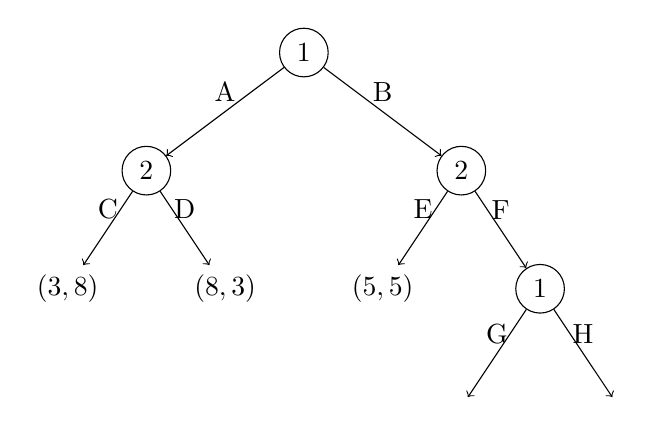
\begin{tikzpicture}[node/.style={draw, circle}]
        \node[node] (p1_a1) at (0,0) {1};
        \node[node] (p2_a1) at (-2,-1.5) {2};
        \node[node] (p2_a2) at (2,-1.5) {2};
        \node[node] (p1_a2) at (3,-3) {1};

        \node[draw=none] (outcome_1) at (-3,-3) {\( (3,8) \)};
        \node[draw=none] (outcome_2) at (-1,-3) {\( (8,3) \)};
        \node[draw=none] (outcome_3) at (1,-3) {\( (5,5) \)};
        \node[draw=none] (outcome_4) at (2,-4.5) {};
        \node[draw=none] (outcome_5) at (4,-4.5) {};

        \draw[->] (p1_a1) -- (p2_a1) node[midway, above] {A};
        \draw[->] (p1_a1) -- (p2_a2) node[midway, above] {B};
        \draw[->] (p2_a1) -- (outcome_1) node[midway, above] {C};
        \draw[->] (p2_a1) -- (outcome_2) node[midway, above] {D};
        \draw[->] (p2_a2) -- (outcome_3) node[midway, above] {E};
        \draw[->] (p2_a2) -- (p1_a2) node[midway, above] {F};
        \draw[->] (p1_a2) -- (outcome_4) node[midway, above] {G};
        \draw[->] (p1_a2) -- (outcome_5) node[midway, above] {H};
    \end{tikzpicture}
\end{frame}


\begin{frame}
    \frametitle{Perfect Information Extensive Form Games}
    \centering
    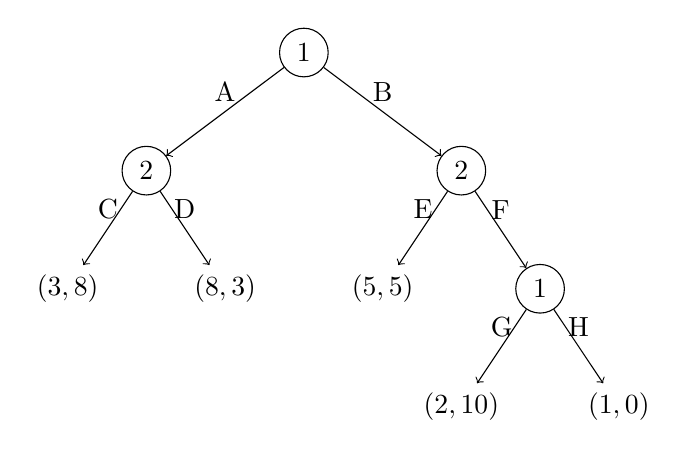
\begin{tikzpicture}[node/.style={draw, circle}]
        \node[node] (p1_a1) at (0,0) {1};
        \node[node] (p2_a1) at (-2,-1.5) {2};
        \node[node] (p2_a2) at (2,-1.5) {2};
        \node[node] (p1_a2) at (3,-3) {1};

        \node[draw=none] (outcome_1) at (-3,-3) {\( (3,8) \)};
        \node[draw=none] (outcome_2) at (-1,-3) {\( (8,3) \)};
        \node[draw=none] (outcome_3) at (1,-3) {\( (5,5) \)};
        \node[draw=none] (outcome_4) at (2,-4.5) {\( (2,10) \)};
        \node[draw=none] (outcome_5) at (4,-4.5) {\( (1,0) \)};

        \draw[->] (p1_a1) -- (p2_a1) node[midway, above] {A};
        \draw[->] (p1_a1) -- (p2_a2) node[midway, above] {B};
        \draw[->] (p2_a1) -- (outcome_1) node[midway, above] {C};
        \draw[->] (p2_a1) -- (outcome_2) node[midway, above] {D};
        \draw[->] (p2_a2) -- (outcome_3) node[midway, above] {E};
        \draw[->] (p2_a2) -- (p1_a2) node[midway, above] {F};
        \draw[->] (p1_a2) -- (outcome_4) node[midway, above] {G};
        \draw[->] (p1_a2) -- (outcome_5) node[midway, above] {H};
    \end{tikzpicture}
\end{frame}
% Turn-based
% Tree
% Players have full knowledge 
% History makes sense
